\documentclass[11pt,a4paper]{article}
\usepackage{fontspec}
\usepackage[spanish,es-tabla,es-nodecimaldot]{babel}
\usepackage[a4paper,top=2.2cm,bottom=2.2cm,left=2.3cm,right=2.3cm]{geometry}
\usepackage{amsmath,amssymb}
\usepackage{xcolor}
\usepackage{longtable,booktabs,array,tabularx,multirow}
\usepackage{graphicx}
\graphicspath{{Imagenes_DCF_IR_LATEX/}}
\usepackage{hyperref}
\usepackage{fancyhdr}
\usepackage{titlesec}
\usepackage{enumitem}
\usepackage{parskip}
\usepackage{caption}
\usepackage{float}
\usepackage{pdflscape}
\usepackage{tikz}
\usetikzlibrary{positioning,arrows.meta,shapes.geometric,fit}
\usepackage{pgfplots}
\pgfplotsset{compat=1.18}
\usepackage[expansion=false]{microtype}
\usepackage{appendix}
\usepackage{lastpage}

\definecolor{uteqgreen}{RGB}{0,102,51}
\definecolor{uteqgold}{RGB}{174,137,47}
\definecolor{lightgray}{RGB}{245,245,245}

\hypersetup{colorlinks=true,linkcolor=black,citecolor=uteqgreen,urlcolor=blue,pdftitle={PE5 - SICM},pdfauthor={Equipo PFC SICM - UTEQ}}

\pagestyle{fancy}\fancyhf{}\fancyhead[L]{\small PE5 - Sistema de Gestión Inteligente para un Centro Médico}\fancyhead[R]{\small UTEQ - ISR-401}\fancyfoot[C]{\thepage}\renewcommand{\headrulewidth}{0.2pt}


\titleformat{\section}
{\Large\bfseries\color{black}}
{\thesection}
{0.8em}
{}

\titleformat{\subsection}
{\large\bfseries\color{black}}
{\thesubsection}
{0.8em}
{}
\setcounter{secnumdepth}{3}\setcounter{tocdepth}{3}
\setlength{\LTleft}{0pt}\setlength{\LTright}{0pt}
\setlength{\tabcolsep}{3pt}
\sloppy
\newcolumntype{Y}{>{\raggedright\arraybackslash}X}
\newcommand{\good}{\textbf{Cumple}}

\begin{document}
	\begin{titlepage}\centering
		{\LARGE\bfseries UNIVERSIDAD TÉCNICA ESTATAL DE \\[0.5cm]
			QUEVEDO    }\\[0.95cm]
		{\large Facultad de Ciencias de la Computación - Carrera de Software}\\[1.0cm]
		{\Large\bfseries PRÁCTICA EXPERIMENTAL\\
			 PE5 - UNIDAD V}\\[0.25cm]
		{\large Integración, Métricas y Defensa del Proyecto Integrador de Ingeniería de Requisitos}\\[0.9cm]
		{\LARGE\bfseries Sistema de Gestión Inteligente para un Centro Médico (SICM)}\\[0.95cm]
		{\large ERS/SRS final conforme a ISO/IEC/IEEE 29148:2018 e ISO/IEC 25010:2023}\\[1cm]
		
				{\large Integrantes del grupo}\\[1cm]
		
		\begin{tabular}{c}
			\textbf{Díaz Pontón Steven Santiago}\\
			\textbf{Tigasi Sampedro Paul Alexander}\\
			\textbf{Vera Gómez Anthony Alfredo}
		\end{tabular}\\[0.9cm]
		
		\begin{tabular}{ll}\textbf{Curso:}&4to Nivel\\\textbf{Asignatura:}&Ingeniería de Requerimientos (ISR-401)\\\textbf{Docente:}&Ing. Gleiston Cicerón Guerrero Ulloa\\\textbf{Versión PE5:}&4.0 - 16/08/2026\end{tabular}\\[0.8cm]
		{\small\textbf{Repositorio GitHub:} \url{https://github.com/ptigasis-Alexander/MediCita_ISR401/tree/main}}\\[0.3cm]
		{\small\textbf{Commit base auditado:} historial público vigente al 16/08/2026. El hash de la línea base PE5 debe corresponder al commit que incorpore estos archivos, por lo que no se fabrica un identificador antes de publicarlos.}\\
		\vfill Quevedo - Los Ríos - Ecuador\\16 de agosto de 2026
	\end{titlepage}
	
\section*{Historial de versiones}
\begin{longtable}{p{1.2cm}p{2cm}p{2.4cm}p{9cm}}
	\toprule\textbf{Versión}&\textbf{Fecha}&\textbf{Entrega}&\textbf{Descripción}\\\midrule\endhead
	1.0&31/05/2026&PE1&Planificación y elicitación base.\\
	2.0&12/07/2026&PE2&Especificación, interfaces, RF/RNF, priorización y trazabilidad parcial.\\
	3.0&26/07/2026&PE3&Ampliación de requisitos, historias de usuario, casos de uso y matriz extendida.\\
	3.1&01/08/2026&Revisión&Normalización del catálogo y concordancia previa.\\
	4.0&16/08/2026&PE5&Integración final: auditoría M1--M6, corrección de defectos residuales, trazabilidad end-to-end, dos componentes IA, retrospectiva y anexos de defensa.\\\bottomrule
\end{longtable}
\section*{Resumen}
El presente informe consolida el Proyecto Fin de Curso de Ingeniería de Requisitos del Sistema de Gestión Inteligente para un Centro Médico (SICM) y ejecuta el cierre solicitado en la Práctica Experimental PE5. El trabajo integra la evidencia de elicitación, el catálogo de requisitos, los modelos UML, la validación, el control de cambios y la trazabilidad en una línea base única. La auditoría inicial identificó debilidades de completitud, verificabilidad, trazabilidad y consistencia: la versión previa contenía 40 requisitos funcionales y 17 no funcionales activos, pero varios requisitos conservaban textos de fusión contradictorios, no todos poseían criterios BDD y la matriz no registraba la cadena completa exigida. La corrección PE5 deja 73 requisitos activos, incluidos dos componentes de inteligencia artificial: un asistente virtual administrativo y un predictor de riesgo de inasistencia usado únicamente para adaptar recordatorios. Ambos incluyen requisitos de rendimiento, equidad, explicabilidad, datos, privacidad, supervisión humana y monitoreo. Después de la corrección, M1a, M1b, M1c, M3, M4ade y M4atr alcanzan 100 \%, M2 alcanza 1,0000, M5 obtiene 2,8 requisitos afectados en promedio y M6 queda en 0,0000. Estos valores corresponden exclusivamente a la auditoría documental del ERS; no representan resultados de desempeño de los modelos de IA ni pruebas de usabilidad del software. La propuesta mantiene el criterio clínico humano y documenta la evidencia necesaria para defensa y reproducción del informe desde LaTeX.\\[0.25cm]
\textbf{Palabras clave:} ingeniería de requisitos, ERS, trazabilidad, métricas, inteligencia artificial, centro médico, PE5.
\clearpage
\section*{Abstract}
This report consolidates the Requirements Engineering Final Course Project for the Intelligent Management System for a Medical Center (SICM) and performs the closure required by Experimental Practice PE5. The work integrates elicitation evidence, the requirements catalogue, UML models, validation, change control, and traceability into a single baseline. The initial audit identified weaknesses in completeness, verifiability, traceability, and consistency: the previous version contained 40 functional requirements and 17 active non-functional requirements, but several requirements still included contradictory merger statements, not every requirement had a BDD acceptance criterion, and the matrix did not record the complete trace chain required by PE5. The corrected baseline contains 73 active requirements, including two artificial-intelligence components: an administrative virtual assistant and a no-show risk predictor used only to adapt appointment reminders. Both include measurable requirements for performance, fairness, explainability, data, privacy, human oversight, and monitoring. After correction, M1a, M1b, M1c, M3, M4 forward, and M4 backward reach 100 percent; M2 reaches 1.0000; M5 yields an average impact of 2.8 requirements; and M6 reaches 0.0000. These values refer only to the documentary audit of the SRS; they are not measured performance results of the AI models or software-usability tests. The design preserves human clinical judgment and documents the evidence needed for technical defense and reproducible LaTeX compilation.\\[0.25cm]
\textbf{Keywords:} requirements engineering, SRS, traceability, metrics, artificial intelligence, medical center, PE5.
\clearpage
\tableofcontents\clearpage
\listoftables\clearpage
\listoffigures\clearpage
\pagenumbering{arabic}
\section{Introducción}
El SICM surge como respuesta a problemas documentados durante la elicitación del PFC: agendamiento manual, fragmentación de la historia clínica entre áreas, comunicación limitada en las derivaciones y control manual del inventario. La especificación previa consolidó cuarenta requisitos funcionales, diecisiete requisitos no funcionales activos, treinta y cuatro historias de usuario y treinta y tres casos de uso. No obstante, la PE5 no evalúa únicamente la existencia de artefactos: exige demostrar su calidad mediante conteos, cerrar la trazabilidad desde la fuente hasta la prueba, incorporar requisitos completos para sistemas basados en inteligencia artificial y dejar una línea base defendible.

La revisión efectuada sobre la versión previa encontró diez defectos residuales de especificación relacionados con solapamientos de alcance y con la contabilización de RNF. También se comprobó que la matriz heredada era útil como trazabilidad parcial, pero no contenía las columnas Clase UML, Proceso DFD, Estado, Caso de prueba y Estado de la traza exigidas para PE5. En consecuencia, este informe no oculta los hallazgos: presenta el estado inicial, la acción aplicada y la re-medición final, de manera que cada porcentaje pueda ser reconstruido.

\subsection{Problema y contexto}
El centro médico atiende procesos clínicos y administrativos de Medicina General, Odontología, Psicología, Nutrición, Terapia Física, Enfermería, Recepción/Recaudación y Coordinación. El SICM se plantea como una aplicación web centralizada para unificar pacientes, citas, historia clínica, signos vitales, recetas, pagos, turnos, inventario, derivaciones, notificaciones, auditoría y reportes. La digitalización se diseña bajo control de acceso por roles y protección reforzada de datos de salud y de menores.

\subsection{Objetivo general}
Integrar, auditar y dejar defendible la versión final del SICM mediante métricas de calidad del ERS, trazabilidad end-to-end, especificación verificable de dos componentes de IA, re-inspección del catálogo y consolidación de los artefactos PE1--PE5.

\subsection{Objetivos específicos}
\begin{enumerate}[label=OE\arabic*.]
	\item Calcular M1--M6 mediante conteos reproducibles y mostrar el par antes/después.
	\item Completar la cadena Fuente $\rightarrow$ Requisito $\rightarrow$ CU $\rightarrow$ Clase $\rightarrow$ DFD $\rightarrow$ Estado $\rightarrow$ BDD $\rightarrow$ CP $\rightarrow$ Historia.
	\item Mantener cero requisitos funcionales huérfanos y documentar la acción tomada sobre cada cadena previamente incompleta.
	\item Especificar dos componentes de IA con rendimiento, equidad, explicabilidad, datos, privacidad, fallback y monitoreo.
	\item Preparar evidencia y respuestas ancladas en artefactos para la defensa individual.
\end{enumerate}

\subsection{Estructura del informe}
El documento sigue las diez secciones obligatorias de la Guía Ampliada PE5. La ERS se integra en la Sección 3; la Sección 4 resume los modelos; la Sección 5 registra la re-inspección; la Sección 6 presenta gestión y trazabilidad; la Sección 7 desarrolla IA; la Sección 8 calcula las métricas; la Sección 9 documenta la retrospectiva y la Sección 10 contiene cinco conclusiones integradoras.
\clearpage
\section{Metodología de Ingeniería de Requisitos}
\subsection{Proceso seguido de PE1 a PE5}
El proceso se organizó de forma incremental. PE1 estableció el contexto, los stakeholders y la evidencia de elicitación. PE2 transformó necesidades en RF y RNF cuantificables y produjo interfaces, priorización y trazabilidad parcial. PE3 amplió el catálogo con Enfermería y Recepción/Recaudación, incorporó historias BDD y casos de uso adicionales. La etapa de validación y gestión revisó consistencia, defectos y cambios. Finalmente, PE5 ejecuta la auditoría cuantitativa, cierra trazas, especifica IA y prepara la defensa.

\begin{table}[H]\centering\caption{Síntesis del proceso PE1--PE5}\label{tab:proceso}
	\begin{tabularx}{\textwidth}{p{1.2cm}p{3cm}Y Y}\toprule
		\textbf{Etapa}&\textbf{Propósito}&\textbf{Técnicas / decisiones}&\textbf{Artefactos principales}\\\midrule
		PE1&Elicitación y contexto&Entrevistas, cuestionario, observación, codificación temática&Evidencias EV, stakeholders, requisitos crudos\\
		PE2&Especificación&Plantilla de atributos, MoSCoW/Kano, BDD inicial&RF/RNF, mockups, historias, matriz parcial\\
		PE3&Integración de áreas&Segunda ronda de elicitación, WSJF, ampliación UML&40 RF, RNF, 34 US, 33 CU\\
		Validación&Calidad y cambio&Inspección documental, control de duplicidad y acceso&Registro de defectos, decisiones de alcance\\
		PE5&Cierre cuantitativo&Métricas M1--M6, E2E, IA, retrospectiva&ERS 4.0, matriz final, auditoría, defensa\\\bottomrule
\end{tabularx}\end{table}

\subsection{Criterios de calidad}
Se adoptan las propiedades operativas de la guía PE5: completitud, consistencia, verificabilidad, trazabilidad, modificabilidad y corrección. Los umbrales se consideran criterios pedagógicos del curso. La norma ISO/IEC/IEEE 29148:2018 se usa para la calidad de la especificación, ISO/IEC 25010:2023 para el marco de calidad y la literatura de trazabilidad para la relación bidireccional entre evidencia, requisitos y artefactos derivados \cite{iso29148,iso25010,gotel1994,ramesh2001}.

El fundamento aplicado combina cuatro ejes: (i) ISO/IEC/IEEE 29148:2018, para exigir requisitos completos, correctos, consistentes, verificables y trazables; (ii) ISO/IEC 25010:2023, para traducir calidad documental y de producto en métricas auditables; (iii) modelos de trazabilidad de requisitos, porque un RF sin fuente o sin prueba pierde utilidad para gestión de cambio; y (iv) literatura de requisitos para sistemas de aprendizaje automático, que obliga a fijar datos, métrica, umbral, equidad, explicabilidad y monitoreo desde la especificación y no después de la implementación \cite{pohl,swebok,vogelsang2019,ahmad2023,habibullah2023}.

\subsection{Regla de autenticidad aplicada}
Los conteos de la auditoría se obtienen del catálogo SICM. No se atribuyen resultados de pruebas de software que no se hayan ejecutado. Los valores que constituyen umbrales de aceptación se identifican como requisitos; los valores de auditoría se calculan únicamente a partir del documento. Para IA, los valores F1, latencia, equidad y disponibilidad son objetivos de aceptación a validar antes de despliegue, no resultados experimentales inventados.

\subsection{Actores formales cubiertos}
Para M1c se normalizan diez actores: Paciente, Médico, Odontología, Psicología, Nutrición, Terapia Física, Enfermería, Recepción/Recaudación, Coordinación/Administración y Sistema de Notificaciones. Todos poseen al menos un RF asociado. Las especialidades clínicas comparten el supertipo Personal Médico en el modelo conceptual, pero se conservan como actores operativos cuando su flujo es distinto.

\subsection{Control de identificadores}
El catálogo previo usa RF-01 a RF-40 y RNF-01 a RNF-16 más RNF-18. RNF-17 no se reutiliza en PE5: queda documentado como identificador retirado/no asignado para evitar renumeraciones que rompan trazabilidad histórica. Los requisitos nuevos de IA usan prefijos RF-IA1, RNF-IA1, RF-IA2 y RNF-IA2.
\clearpage


SECCION DE ERS SRS

\section{Modelos UML y lectura interpretativa}
La PE5 no reemplaza los modelos previos; verifica su coherencia con el catálogo final. Para la integración se incorporan dos vistas resumidas que conectan requisitos, clases y estados. Las figuras se interpretan en el texto y sus elementos aparecen también en la matriz de trazabilidad.

\subsection{Vista resumida de casos de uso}
\begin{figure}[H]\centering
	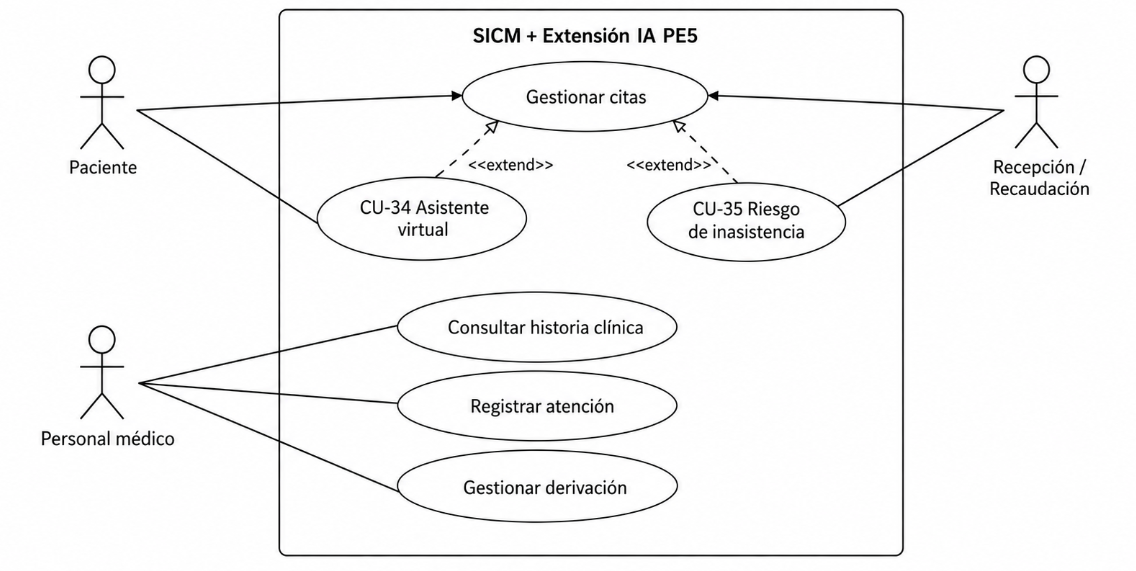
\includegraphics[width=0.95\textwidth]{D_Casos_Uso_R.png}
	\caption{Vista resumida de casos de uso relevantes para la integración PE5.}\label{fig:cu}
\end{figure}



La Figura \ref{fig:cu} muestra que los componentes de IA no quedan aislados: CU-34 se relaciona con el flujo de atención administrativa y CU-35 con citas y notificaciones. Ninguno decide diagnósticos o tratamientos.

\subsection{Modelo conceptual de clases}
\begin{figure}[H]\centering
	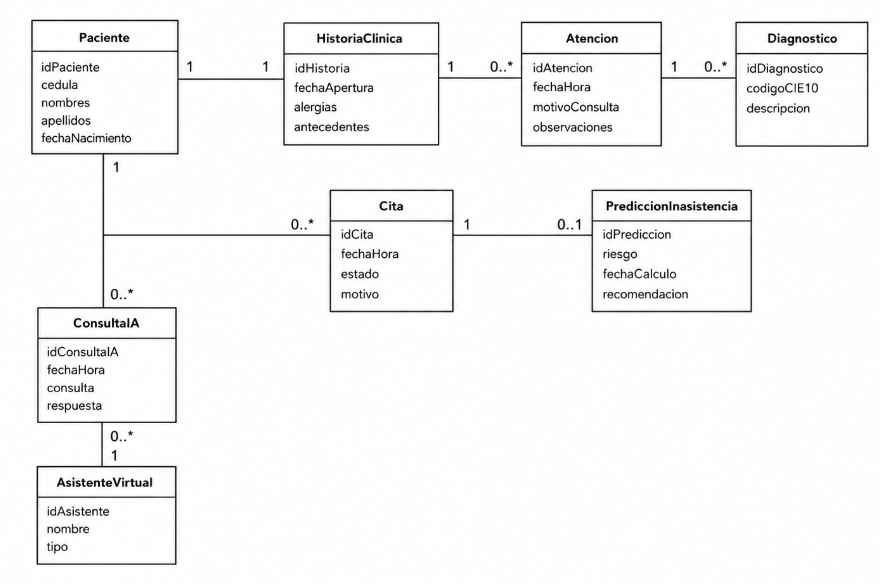
\includegraphics[width=0.90\textwidth]{D_Conceptual.png}
	\caption{Clases conceptuales principales del SICM y extensión IA PE5.}\label{fig:clases}
\end{figure}

\subsection{Estados críticos}
\begin{figure}[H]\centering
	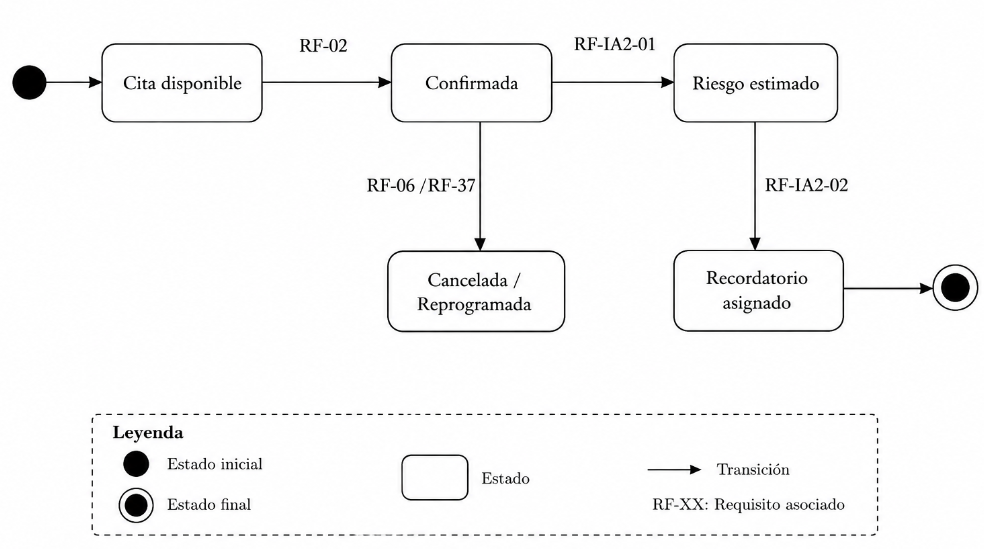
\includegraphics[width=0.95\textwidth]{D_Estado_Critico.png}
	\caption{Fragmento del diagrama de estados de cita con la extensión IA.}\label{fig:estados}
\end{figure}

\subsection{Procesos DFD usados en trazabilidad}
Los procesos normalizados son P00 Autenticar y autorizar, P01 Gestionar pacientes, P02 Gestionar citas, P03 Gestionar historia clínica, P04 Gestionar derivaciones, P05 Gestionar personal, P06 Gestionar inventario, P07 Gestionar recaudación, P08 Generar reportes, P09 Notificar, P10 Auditar, P11 Asistente virtual IA y P12 Estimar riesgo de inasistencia. Esta nomenclatura permite que cada fila de la matriz tenga una referencia explícita y evita la expresión ambigua ``No aplica'' cuando sí existe un proceso lógico.
\clearpage
\section{Validación: inspección, defectos y re-inspección}
\subsection{Método de re-inspección PE5}
Se comparó el catálogo previo con la guía PE5 y se aplicó una revisión sistemática de identificadores, alcance, prioridad, fuente, verificabilidad y trazabilidad. Para consistencia se analizaron los pares del catálogo y se registraron los conflictos de alcance detectados. Para corrección se contabilizaron únicamente defectos residuales de especificación, no errores editoriales externos al requisito.

\begin{longtable}{p{1.5cm}p{2cm}p{2.3cm}p{3.5cm}p{4.5cm}p{1.3cm}}
	\caption{Registro de defectos residuales de especificación PE5}\label{tab:defectos}\\\toprule
	\textbf{ID}&\textbf{Elemento}&\textbf{Tipo}&\textbf{Hallazgo}&\textbf{Corrección aplicada}&\textbf{Estado}\\\midrule\endhead
	D-PE5-01 & RF-01/RF-14 & Solapamiento & RF-01 declaraba a RF-14 fusionado aunque RF-14 seguía activo. & Se separó historia clínica de digitalización de formularios. & Cerrado\\
	D-PE5-02 & RF-02/RF-36 & Solapamiento & RF-02 declaraba absorbido el agendamiento por área. & RF-02 = autoservicio del paciente; RF-36 = operación por área/recepción. & Cerrado\\
	D-PE5-03 & RF-03/RF-27 & Solapamiento & Búsqueda general y búsqueda operativa por cédula aparecían fusionadas. & Se delimitó búsqueda clínica multícriterio y búsqueda rápida de recepción/enfermería. & Cerrado\\
	D-PE5-04 & RF-06/RF-37 & Solapamiento & Cancelación del paciente y reprogramación por área estaban fusionadas. & Se separó por actor y responsabilidad de auditoría. & Cerrado\\
	D-PE5-05 & RF-10/RF-30 & Duplicidad parcial & Gestión de roles incluía restricción clínica que también estaba en RF-30. & RF-10 administra permisos; RF-30 aplica restricción clínica por especialidad. & Cerrado\\
	D-PE5-06 & RF-15/RF-31/RF-32 & Duplicidad parcial & Inventario declaraba absorbidas alerta y entrega trazable. & Se mantuvieron tres responsabilidades independientes y trazables. & Cerrado\\
	D-PE5-07 & RF-18/RF-19 & Solapamiento & Asignación de turnos declaraba fusionada la consulta de disponibilidad. & RF-18 administra turnos; RF-19 consulta disponibilidad. & Cerrado\\
	D-PE5-08 & RF-22/RF-33 & Solapamiento & Pago y cobro por área quedaban sin frontera clara. & RF-22 administra pagos del comprobante; RF-33 habilita flujo de recepción por área. & Cerrado\\
	D-PE5-09 & RF-24/RF-25 & Solapamiento & Configuración horaria declaraba absorbido el cupo máximo. & RF-24 configura horarios; RF-25 controla capacidad por turno. & Cerrado\\
	D-PE5-10 & RNF-01..RNF-18 & Completitud & El texto afirmaba 18 RNF aunque RNF-17 no estaba definido. & Se documentó RNF-17 como identificador retirado/no activo y se fijó el catálogo base en 17 RNF activos. & Cerrado\\
	\bottomrule\end{longtable}

\subsection{Resultado de la re-inspección}
La versión previa tenía diez defectos residuales de especificación entre 57 requisitos activos. Después de delimitar responsabilidades, normalizar el catálogo de RNF y agregar los requisitos PE5 de IA, se ejecutó una segunda revisión sobre 73 requisitos activos. No quedaron conflictos de alcance abiertos en el catálogo generado. Este resultado documental sustenta M6; no debe confundirse con defectos de implementación del software, que pertenecen a pruebas posteriores.

\subsection{Criterio de verificabilidad}
Todo requisito se revisó con cuatro preguntas: existencia de resultado observable o umbral, definición de unidad/estado esperado, escenario o método de comprobación y posibilidad de que dos evaluadores lleguen al mismo veredicto. Los requisitos que no tenían BDD explícito recibieron un escenario BDD asociado en la matriz final.
\clearpage
\section{Gestión, línea base y trazabilidad}
\subsection{Línea base y control de cambios}
La versión PE5 se identifica como 4.0. La línea base válida debe etiquetarse en Git después de incorporar el PDF, el archivo .tex, la matriz CSV, el instrumento de auditoría y el README actualizado. Para evitar una evidencia falsa, este documento no inventa un hash futuro: el hash definitivo debe ser el del commit real que contenga estos artefactos.

\subsection{Diagnóstico de la matriz heredada}
La matriz pública previa contenía 57 filas y relacionaba evidencia, RF/RNF, CU, HU, criterios de aceptación, componentes y mockups. Esa estructura demostraba trazabilidad parcial, pero no permitía calcular M4ade conforme a PE5 porque no registraba de forma explícita Clase UML, Proceso DFD, Estado, Caso de prueba ni Estado de la traza. Por ello el valor inicial de cadena completa se registra como 0/40 RF, sin negar la existencia de enlaces parciales.

\subsection{Matriz end-to-end PE5}
La matriz final contiene 73 filas, una por requisito activo. Para los 45 RF la cadena hacia delante está completa y los 45 poseen fuente identificada. Los RNF también se trazan para facilitar análisis de impacto. La matriz completa se entrega como CSV y se reproduce en el Anexo A en formato legible.

\begin{table}[H]\centering\caption{Cobertura de trazabilidad después de la corrección}\label{tab:trazares}
	\begin{tabular}{lrrr}\toprule\textbf{Indicador}&\textbf{Numerador}&\textbf{Denominador}&\textbf{Cobertura}\\\midrule
		RF con fuente identificada&45&45&100 \%\\
		RF con CU&45&45&100 \%\\
		RF con Clase UML&45&45&100 \%\\
		RF con proceso DFD&45&45&100 \%\\
		RF con Estado/Transición&45&45&100 \%\\
		RF con BDD&45&45&100 \%\\
		RF con CP conceptual&45&45&100 \%\\
		RF con Historia&45&45&100 \%\\\bottomrule\end{tabular}\end{table}

\subsection{Huérfanos y cadenas rotas}
\begin{table}[H]\centering\caption{Cierre de patologías de trazabilidad}\label{tab:huerfanos}
	\begin{tabularx}{\textwidth}{p{3cm}Y Y}\toprule\textbf{Identificador}&\textbf{Causa inicial}&\textbf{Acción tomada}\\\midrule
		RF-16&No tenía CU formal en la matriz previa.&Se especificó CU-34 y se enlazó con US-35, clases de IA, P11, BDD y CP.\\
		RNF sin BDD&Varios RNF se expresaban solo como métrica.&Se creó un escenario BDD conceptual por RNF y su CP correspondiente.\\
		RF de IA PE5&No existían en la versión previa.&Se añadieron con fuente explícita y trazas a RF/CU existentes y a CU-34/CU-35.\\
		Matriz PE3&Carecía de Clase, DFD, Estado y CP.&Se migró a la estructura PE5 y cada fila quedó en estado Completa.\\\bottomrule\end{tabularx}\end{table}

\clearpage

  SECCION 7
\section{Requisitos de Inteligencia Artificial}
\subsection{Principio de diseño}
La IA del SICM se limita a apoyo administrativo. No diagnostica, no prescribe, no realiza triaje de emergencia y no decide si una persona recibe atención. Esta frontera reduce el impacto potencial y mantiene supervisión humana. La ingeniería de requisitos para sistemas de aprendizaje automático exige especificar datos, métricas, contexto de evaluación, equidad, explicabilidad y monitoreo, porque el comportamiento depende del conjunto de datos y no es completamente determinista \cite{vogelsang2019,ahmad2023,habibullah2023}. 
	SECCION DE METRICAS 
	
\section{Retrospectiva Start--Stop--Continue}
La retrospectiva se centra en hechos observables del proyecto: ampliaciones tardías del catálogo, duplicidades de alcance, existencia de evidencia de elicitación y uso sostenido de control de versiones.
\begin{longtable}{p{2.2cm}p{8cm}p{5.5cm}}
	\caption{Retrospectiva PE5 con responsables}\label{tab:retro}\\\toprule\textbf{Categoría}&\textbf{Elemento}&\textbf{Responsable / acción}\\\midrule\endhead
	Start&Ejecutar un validador de identificadores, referencias y trazas en cada entrega.&Líder + Técnico: incluir revisión antes de cada baseline.\\
	Start&Calcular M1--M6 desde versiones intermedias para detectar faltantes antes del cierre.&Verificación: mantener hoja de conteos versionada.\\
	Start&Definir requisitos de IA con datos, equidad y fallback desde que se propone el componente.&Equipo completo: usar ficha IA como criterio de entrada.\\
	Stop&Declarar que un requisito fue ``fusionado'' mientras el identificador absorbido continúa activo.&Analista: cualquier fusión exige RFC, actualización de matriz y retiro explícito.\\
	Stop&Usar ``No aplica'' como sustituto de una traza que sí puede identificarse.&Modelado: registrar proceso/clase/estado o justificar realmente la no aplicabilidad.\\
	Stop&Dejar requisitos cuantificados sin BDD asociado.&Verificación: ningún requisito entra a la línea base sin método de comprobación.\\
	Continue&Realizar elicitación con personal de múltiples áreas clínicas y administrativas.&Equipo de elicitación: conservar evidencia y consentimiento.\\
	Continue&Usar GitHub para versionar ERS, modelado y trazabilidad.&Líder: etiquetar líneas base y revisar distribución de commits.\\
	Continue&Redactar RNF con unidades y umbrales en lugar de términos vagos.&Documentación + verificación: aplicar checklist 29148/25010.\\\bottomrule\end{longtable}
\clearpage

  SECCION 10
  
\section*{Referencias}\addcontentsline{toc}{section}{Referencias}
\begin{thebibliography}{99}
	\bibitem{iso29148} ISO/IEC/IEEE, \emph{ISO/IEC/IEEE 29148:2018 Systems and software engineering--Life cycle processes--Requirements engineering}, 2018.
	\bibitem{iso25010} ISO/IEC, \emph{ISO/IEC 25010:2023 Systems and software engineering--SQuaRE--Product quality model}, 2023.
	\bibitem{gotel1994} O. C. Z. Gotel and A. C. W. Finkelstein, ``An analysis of the requirements traceability problem,'' in \emph{Proc. IEEE ICRE}, 1994, pp. 94--101, doi: 10.1109/ICRE.1994.292398.
	\bibitem{ramesh2001} B. Ramesh and M. Jarke, ``Toward reference models for requirements traceability,'' \emph{IEEE Trans. Software Engineering}, vol. 27, no. 1, pp. 58--93, 2001, doi: 10.1109/32.895989.
	\bibitem{pohl} K. Pohl, \emph{Requirements Engineering: Fundamentals, Principles, and Techniques}, 2nd ed. Springer, 2025, ISBN 978-3-662-69204-2.
	\bibitem{swebok} H. Washizaki, Ed., \emph{Guide to the Software Engineering Body of Knowledge, Version 4.0}. IEEE Computer Society, 2024.
	\bibitem{vogelsang2019} A. Vogelsang and M. Borg, ``Requirements engineering for machine learning: Perspectives from data scientists,'' in \emph{2019 IEEE REW}, pp. 245--251, doi: 10.1109/REW.2019.00050.
	\bibitem{ahmad2023} K. Ahmad, M. Abdelrazek, C. Arora, M. Bano, and J. Grundy, ``Requirements engineering for artificial intelligence systems: A systematic mapping study,'' \emph{Information and Software Technology}, vol. 158, 107176, 2023, doi: 10.1016/j.infsof.2023.107176.
	\bibitem{habibullah2023} K. M. Habibullah, G. Gay, and J. Horkoff, ``Non-functional requirements for machine learning,'' \emph{Requirements Engineering}, vol. 28, pp. 283--316, 2023, doi: 10.1007/s00766-022-00395-3.
	\bibitem{loppd} República del Ecuador, \emph{Ley Orgánica de Protección de Datos Personales}, Registro Oficial, Quinto Suplemento No. 459, 26 mayo 2021.
	\bibitem{euaiact2024} European Parliament and Council of the European Union, \emph{Regulation (EU) 2024/1689 laying down harmonised rules on artificial intelligence}, Official Journal of the European Union, 2024.
	\bibitem{whoai2021} World Health Organization, \emph{Ethics and Governance of Artificial Intelligence for Health}. Geneva: WHO, 2021, ISBN 978-92-4-002920-0.
	\bibitem{topol2019} E. J. Topol, ``High-performance medicine: the convergence of human and artificial intelligence,'' \emph{Nature Medicine}, vol. 25, pp. 44--56, 2019, doi: 10.1038/s41591-018-0300-7.
	\bibitem{hayrinen2008} K. Häyrinen, K. Saranto, and P. Nykänen, ``Definition, structure, content, use and impacts of electronic health records,'' \emph{Int. J. Med. Inform.}, vol. 77, no. 5, pp. 291--304, 2008, doi: 10.1016/j.ijmedinf.2008.01.001.
	\bibitem{menachemi2011} N. Menachemi and T. H. Collum, ``Benefits and drawbacks of electronic health record systems,'' \emph{Risk Management and Healthcare Policy}, vol. 4, pp. 47--55, 2011, doi: 10.2147/RMHP.S12985.
\end{thebibliography}
\clearpage
\begin{appendices}
	\section{Instrumento de auditoría y matriz final}
	\subsection{Instrumento de auditoría}
	La Tabla \ref{tab:auditoria} constituye el instrumento aplicado. Los archivos entregables incluyen además \texttt{instrumento\_auditoria\_PE5.csv} con la misma aritmética para revisión independiente.
	
	
	\subsection{Catálogo BDD complementario para RNF e IA}
	La matriz señala el identificador BDD de cada requisito. Los 40 RF heredados conservan su BDD dentro de la ficha funcional; la Tabla \ref{tab:bddcomplementario} explicita los escenarios que completan la evidencia para los 17 RNF base, los cinco RF nuevos de IA y los once RNF nuevos de IA. Los valores cuantitativos de producto se interpretan como umbrales de aceptación según la Sección \ref{subsec:umbrales-ia}.
	\scriptsize
	\begin{longtable}{p{2.8cm}p{10.6cm}p{2cm}}
		\caption{BDD complementarios de RNF y requisitos de IA}\label{tab:bddcomplementario}\\
		\toprule\textbf{ID BDD}&\textbf{Escenario Dado-Cuando-Entonces}&\textbf{CP}\\\midrule
		\endfirsthead
		\multicolumn{3}{c}{\small\textit{Tabla \thetable\ -- continuación}}\\
		\toprule\textbf{ID BDD}&\textbf{Escenario Dado-Cuando-Entonces}&\textbf{CP}\\\midrule
		\endhead
		BDD-RNF-01 & Dado que hasta 50 usuarios concurrentes consultan historiales clínicos, cuando se mide el tiempo de respuesta, entonces al menos el 95 \% de las consultas debe completarse en 2 s o menos. & CP-RNF-01\\
		BDD-RNF-02 & Dado que se transmiten y almacenan datos clínicos en el ambiente de prueba, cuando se verifican los controles de seguridad, entonces la comunicación usa TLS 1.2 o superior, el almacenamiento usa AES-256 y los accesos no autorizados son rechazados. & CP-RNF-02\\
		BDD-RNF-03 & Dado un grupo de usuarios de validación y tareas representativas del SICM, cuando se ejecuta la prueba de usabilidad, entonces la tasa de finalización debe ser al menos 90 \% y la puntuación SUS al menos 75/100. & CP-RNF-03\\
		BDD-RNF-04 & Dado el horario institucional de 07h00 a 18h00 de lunes a viernes, cuando se monitorea la operación durante el periodo definido, entonces la disponibilidad debe ser al menos 99 \% y el MTTR no superar 30 min. & CP-RNF-04\\
		BDD-RNF-05 & Dado un cambio funcional aprobado, cuando se ejecuta la compilación y la suite automatizada, entonces la cobertura debe ser al menos 70 \% y el cambio debe quedar confinado a los módulos previstos por la arquitectura. & CP-RNF-05\\
		BDD-RNF-06 & Dado un usuario sin autorización sobre una historia clínica, cuando intenta acceder al recurso protegido, entonces el acceso debe ser rechazado y el evento registrado en auditoría en el 100 \% de los casos de prueba. & CP-RNF-06\\
		BDD-RNF-07 & Dado cada navegador y resolución declarados, cuando se recorren los flujos críticos del SICM, entonces las funciones deben operar sin pérdida de contenido ni acciones inaccesibles. & CP-RNF-07\\
		BDD-RNF-08 & Dado un conjunto de expedientes válidos, cuando se consulta por cédula, entonces al menos el 95 \% de las búsquedas debe devolver el expediente en 3 s o menos. & CP-RNF-08\\
		BDD-RNF-09 & Dado el periodo mensual de operación de Enfermería y Recepción, cuando se calcula el tiempo disponible del servicio, entonces la disponibilidad debe ser al menos 99 \%. & CP-RNF-09\\
		BDD-RNF-10 & Dado un usuario de una especialidad sin permiso sobre información clínica de otra área, cuando intenta consultarla, entonces el 100 \% de los accesos no autorizados debe bloquearse y registrarse en bitácora. & CP-RNF-10\\
		BDD-RNF-11 & Dado un registro clínico guardado en un módulo origen, cuando otro módulo autorizado consulta la actualización, entonces los datos deben propagarse en 10 s o menos. & CP-RNF-11\\
		BDD-RNF-12 & Dado un usuario sin experiencia previa que recibió 1 h de capacitación, cuando registra un paciente nuevo, entonces debe completar la tarea en 5 min o menos con una tasa de error no superior al 5 \%. & CP-RNF-12\\
		BDD-RNF-13 & Dado un formulario de paciente con campos obligatorios, cuando se intenta guardar información inválida o incompleta, entonces el sistema la rechaza; todo registro aceptado debe cumplir el 100 \% de las validaciones definidas. & CP-RNF-13\\
		BDD-RNF-14 & Dado el inventario de equipos actuales del centro, cuando se ejecutan los flujos esenciales del SICM en cada equipo, entonces el 100 \% debe funcionar sin requerir ampliación obligatoria de hardware. & CP-RNF-14\\
		BDD-RNF-15 & Dado el conjunto operativo de inventario, cuando un usuario autorizado solicita el informe, entonces la generación completa debe finalizar en 2 min o menos. & CP-RNF-15\\
		BDD-RNF-16 & Dado un conjunto de casos de menores y representantes con identidades diferenciadas, cuando se registra y consulta la relación, entonces no debe producirse ninguna asociación errónea en los casos de prueba. & CP-RNF-16\\
		BDD-RNF-18 & Dado que el asistente deriva una consulta a recepción, cuando presenta la explicación al paciente, entonces debe mostrarla en 2 s o menos, usar como máximo 40 palabras y alcanzar al menos 80 \% de valoraciones de 4/5 o más en la validación definida. & CP-RNF-18\\
		BDD-RF-IA1-02 & Dado una consulta administrativa dentro del alcance, cuando el asistente la procesa, entonces debe clasificarla en una intención definida y utilizar una fuente institucional aprobada. & CP-RF-IA1-02\\
		BDD-RF-IA1-03 & Dado una consulta clínica, ambigua o fuera de alcance, cuando el asistente detecta esa condición, entonces debe derivarla a recepción sin emitir diagnóstico ni recomendación clínica autónoma. & CP-RF-IA1-03\\
		BDD-RNF-IA1-P01 & Dado el conjunto de prueba versionado de intenciones administrativas, cuando se evalúa el clasificador, entonces el macro-F1 debe ser al menos 0.90. & CP-RNF-IA1-P01\\
		BDD-RNF-IA1-P02 & Dado 50 sesiones concurrentes, cuando el asistente responde o decide escalar una consulta, entonces la latencia P95 debe ser 2 s o menor. & CP-RNF-IA1-P02\\
		BDD-RNF-IA1-P03 & Dado el horario de atención, cuando se monitorea el servicio del asistente, entonces la disponibilidad debe ser al menos 99 \% y, ante fallo, el fallback a recepción debe mostrarse en 2 s o menos. & CP-RNF-IA1-P03\\
		BDD-RNF-IA1-E01 & Dado una muestra de evaluación con usuarios de 18-35 años y mayores de 60, cuando se calcula la tasa de resolución correcta por grupo, entonces la diferencia no debe superar 5 puntos porcentuales. & CP-RNF-IA1-E01\\
		BDD-RNF-IA1-E02 & Dado una muestra con usuarios de baja y alta familiaridad digital, cuando se compara la tasa de resolución correcta, entonces la diferencia no debe superar 5 puntos porcentuales. & CP-RNF-IA1-E02\\
		BDD-RF-IA2-01 & Dado una cita confirmada con datos administrativos permitidos, cuando se solicita la predicción, entonces el sistema debe generar un puntaje de riesgo de inasistencia entre 0 y 1 sin usar datos clínicos. & CP-RF-IA2-01\\
		BDD-RF-IA2-02 & Dado un puntaje de riesgo generado, cuando el sistema selecciona una estrategia de recordatorio, entonces debe clasificar el riesgo y no cancelar, negar ni reducir la prioridad clínica de la cita. & CP-RF-IA2-02\\
		BDD-RF-IA2-03 & Dado una predicción disponible para una cita, cuando recepción decide anularla o aplicar una estrategia manual, entonces el sistema debe respetar la decisión humana y registrar la acción en auditoría. & CP-RF-IA2-03\\
		BDD-RNF-IA2-P01 & Dado el conjunto de prueba temporal definido antes del despliegue, cuando se evalúa el predictor de inasistencia, entonces el F1 debe ser al menos 0.80. & CP-RNF-IA2-P01\\
		BDD-RNF-IA2-P02 & Dado un lote de hasta 100 citas, cuando se ejecuta la inferencia, entonces la latencia P95 debe ser 500 ms o menor. & CP-RNF-IA2-P02\\
		BDD-RNF-IA2-P03 & Dado el servicio predictivo en horario operativo, cuando se monitorea su disponibilidad, entonces debe alcanzar al menos 99 \% y, si falla, conservar el recordatorio estándar sin afectar la cita. & CP-RNF-IA2-P03\\
		BDD-RNF-IA2-E01 & Dado una muestra de evaluación con usuarios de 18-35 años y mayores de 60, cuando se calcula la sensibilidad por grupo, entonces la diferencia no debe superar 5 puntos porcentuales. & CP-RNF-IA2-E01\\
		BDD-RNF-IA2-E02 & Dado una muestra con pacientes nuevos y recurrentes, cuando se calcula la tasa de falsos positivos por grupo, entonces la diferencia no debe superar 5 puntos porcentuales. & CP-RNF-IA2-E02\\
		BDD-RNF-IA2-X01 & Dado un riesgo medio o alto mostrado a recepción, cuando se presenta la predicción, entonces el sistema debe indicar al menos dos factores administrativos influyentes y advertir que la predicción no modifica la atención. & CP-RNF-IA2-X01\\
		\bottomrule\end{longtable}
	\normalsize
	
	\subsection{Matriz de trazabilidad completa}
	Por legibilidad, la matriz se imprime en orientación horizontal. El CSV asociado es el artefacto principal para filtrado y auditoría.
	\begin{landscape}\scriptsize
		\begin{longtable}{p{2.2cm}p{1.8cm}p{2cm}p{3cm}p{3cm}p{3cm}p{2cm}p{2cm}p{2cm}p{1.6cm}}
			\caption{Matriz end-to-end PE5 (73 requisitos)}\\\toprule
			\textbf{Fuente}&\textbf{Req.}&\textbf{CU}&\textbf{Clase UML}&\textbf{Proceso DFD}&\textbf{Estado}&\textbf{BDD}&\textbf{CP}&\textbf{Historia}&\textbf{Traza}\\\midrule\endhead
			Acta de entrevista N°1 (EV-01) & RF-01 & CU-02 & Paciente, HistoriaClinica & P03 Gestionar historia clínica & Sin historia -> Historia activa & BDD-RF-01 & CP-RF-01 & US-06 & Completa\\
			Acta de entrevista N°1, Cuestionario digital (EV-01, EV-02) & RF-02 & CU-01 & Paciente, Cita, Horario & P02 Gestionar citas & Disponible -> Reservada -> Confirmada & BDD-RF-02 & CP-RF-02 & US-01 & Completa\\
			Acta de entrevista N°1 (EV-01) & RF-03 & CU-02 & Paciente, HistoriaClinica & P01 Gestionar pacientes & Consulta iniciada -> Paciente encontrado/no encontrado & BDD-RF-03 & CP-RF-03 & US-02 & Completa\\
			Médico (Odontología / Medicina General) / Acta de entrevista N°1 (EV-01) & RF-04 & CU-03 & Receta, Medicamento, HistoriaClinica & P03 Gestionar historia clínica & Atención activa -> Receta emitida & BDD-RF-04 & CP-RF-04 & US-03 & Completa\\
			Acta de entrevista N°1 (EV-01) & RF-05 & CU-02 & HistoriaClinica, Auditoria & P03 Gestionar historia clínica & Historia activa -> Actualizada & BDD-RF-05 & CP-RF-05 & US-05 & Completa\\
			Acta de entrevista N°1 (EV-01) & RF-06 & CU-04 & Cita, Horario & P02 Gestionar citas & Confirmada -> Reprogramada/Cancelada & BDD-RF-06 & CP-RF-06 & US-04 & Completa\\
			Acta de negociación N°1 (EV-04) & RF-07 & CU-05 & Derivacion, HistoriaClinica, AreaMedica & P04 Gestionar derivaciones & Atención -> Derivada -> Aceptada & BDD-RF-07 & CP-RF-07 & US-19 & Completa\\
			Administrador / Acta de entrevista N°1 (EV-01) & RF-08 & CU-05 & Atencion, Reporte & P08 Generar reportes & Solicitud -> Reporte generado & BDD-RF-08 & CP-RF-08 & US-06 & Completa\\
			EV-01 / CU-12 & RF-09 & CU-12/CU-32/CU-33 & Usuario, Sesion & P00 Autenticar y autorizar & No autenticado -> Autenticado/Bloqueado & BDD-RF-09 & CP-RF-09 & US-07/US-31/US-32 & Completa\\
			EV-04 & RF-10 & CU-13/CU-31 & Usuario, Rol, Permiso & P00 Autenticar y autorizar & Rol vigente -> Rol actualizado & BDD-RF-10 & CP-RF-10 & US-08/US-30 & Completa\\
			Cuestionario digital (EV-02): 100 \% prefiere WhatsApp & RF-11 & CU-14 & Notificacion, Cita & P09 Notificar & Pendiente -> Enviada/Fallida & BDD-RF-11 & CP-RF-11 & US-01 & Completa\\
			Acta de negociación N°1 (EV-04) & RF-12 & CU-15 & Auditoria, Usuario & P10 Auditar & Evento -> Registrado & BDD-RF-12 & CP-RF-12 & US-09 & Completa\\
			Diagrama de CU-01 Agendar cita médica (Figura 12) & RF-13 & CU-01 & Horario, Cita & P02 Gestionar citas & Sin horario -> Horario disponible & BDD-RF-13 & CP-RF-13 & US-01 & Completa\\
			EV-01 & RF-14 & CU-22 & DocumentoClinico, HistoriaClinica & P03 Gestionar historia clínica & Físico -> Digital validado & BDD-RF-14 & CP-RF-14 & US-05 & Completa\\
			EV-Enf-01 & RF-15 & CU-29 & Inventario, Medicamento, MovimientoInventario & P06 Gestionar inventario & Disponible -> Actualizado/Stock bajo & BDD-RF-15 & CP-RF-15 & US-33 & Completa\\
			EV-01 & RF-16 & CU-34 & AsistenteVirtual, ConsultaIA & P11 Asistente virtual IA & Consulta -> Respondida/Derivada & BDD-RF-16 & CP-RF-16 & US-35 & Completa\\
			Coordinadora del centro médico & RF-17 & CU-16 & Profesional, AreaMedica & P05 Gestionar personal & No registrado -> Perfil activo & BDD-RF-17 & CP-RF-17 & US-10 & Completa\\
			Jefatura de área médica & RF-18 & CU-17 & Profesional, TurnoLaboral & P05 Gestionar personal & Sin turno -> Turno asignado & BDD-RF-18 & CP-RF-18 & US-11 & Completa\\
			Paciente (módulo de agendamiento) & RF-19 & CU-17 & Profesional, TurnoLaboral & P05 Gestionar personal & Ocupado/Libre & BDD-RF-19 & CP-RF-19 & US-12 & Completa\\
			Personal médico & RF-20 & CU-17 & Profesional, Ausencia, TurnoLaboral & P05 Gestionar personal & Activo -> Ausente -> Reasignado & BDD-RF-20 & CP-RF-20 & US-11 & Completa\\
			Requisito normativo SRI & RF-21 & CU-18 & Comprobante, Paciente & P07 Gestionar recaudación & Servicio -> Comprobante emitido & BDD-RF-21 & CP-RF-21 & US-13 & Completa\\
			EV-Enf-01 & RF-22 & CU-19 & Pago, Comprobante & P07 Gestionar recaudación & Pendiente -> Parcial/Pagado & BDD-RF-22 & CP-RF-22 & US-14 & Completa\\
			EV-Enf-01 & RF-23 & CU-19 & Pago, ReporteFinanciero & P08 Generar reportes & Solicitud -> Reporte financiero & BDD-RF-23 & CP-RF-23 & US-14 & Completa\\
			EV-01 & RF-24 & CU-11 & AreaMedica, Horario & P02 Gestionar citas & Horario base -> Configurado & BDD-RF-24 & CP-RF-24 & US-15 & Completa\\
			EV-01 & RF-25 & CU-11 & Horario, Cupo & P02 Gestionar citas & Cupo disponible -> Cupo completo & BDD-RF-25 & CP-RF-25 & US-15 & Completa\\
			Entrevista al personal de Enfermería y Recepción & RF-26 & CU-06 & SignosVitales, Paciente & P03 Gestionar historia clínica & Pendiente -> Signos registrados & BDD-RF-26 & CP-RF-26 & US-16 & Completa\\
			Recepcionista / Entrevista al personal de Enfermería y Recepción & RF-27 & CU-07 & Paciente, HistoriaClinica & P01 Gestionar pacientes & Consulta -> Encontrado & BDD-RF-27 & CP-RF-27 & US-17 & Completa\\
			Recepcionista / Entrevista al personal de Enfermería y Recepción & RF-28 & CU-07/CU-20 & Paciente, Representante & P01 Gestionar pacientes & No registrado -> Registrado & BDD-RF-28 & CP-RF-28 & US-18 & Completa\\
			Recepcionista / Entrevista al personal de Enfermería y Recepción & RF-29 & CU-20 & Paciente, Representante & P01 Gestionar pacientes & Menor sin ID -> Vinculado & BDD-RF-29 & CP-RF-29 & US-18 & Completa\\
			Administrador del sistema / Entrevista al personal de Enfermería y Recepción & RF-30 & CU-10 & Usuario, Rol, HistoriaClinica & P00 Autenticar y autorizar & Solicitud acceso -> Permitido/Denegado & BDD-RF-30 & CP-RF-30 & US-19 & Completa\\
			Enfermería / EV-Enf-01 & RF-31 & CU-29 & Medicamento, AlertaInventario & P06 Gestionar inventario & Normal -> Alerta activa & BDD-RF-31 & CP-RF-31 & US-33 & Completa\\
			EV-Enf-01 & RF-32 & CU-30 & EntregaMedicamento, Medicamento, Paciente & P06 Gestionar inventario & Prescrito -> Entregado & BDD-RF-32 & CP-RF-32 & US-34 & Completa\\
			EV-Enf-01 & RF-33 & CU-08 & Pago, AreaMedica, Paciente & P07 Gestionar recaudación & Pendiente -> Cobrado & BDD-RF-33 & CP-RF-33 & US-20 & Completa\\
			Recepcionista / Entrevista al personal de Enfermería y Recepción & RF-34 & CU-08 & TurnoAtencion, Paciente & P07 Gestionar recaudación & Cobrado -> Turno asignado & BDD-RF-34 & CP-RF-34 & US-21 & Completa\\
			Profesional del área (destino) / Entrevista al personal de Enfermería y Recepción & RF-35 & CU-09 & Derivacion, AreaMedica, Paciente & P04 Gestionar derivaciones & Enfermería -> Área destino & BDD-RF-35 & CP-RF-35 & US-19 & Completa\\
			Profesional del área / EV-Enf-01 & RF-36 & CU-01 & Cita, AreaMedica, Profesional & P02 Gestionar citas & Disponible -> Cita de área & BDD-RF-36 & CP-RF-36 & US-01 & Completa\\
			Profesional del área / EV-Enf-01 & RF-37 & CU-21 & Cita, Auditoria & P02 Gestionar citas & Activa -> Reprogramada/Cancelada & BDD-RF-37 & CP-RF-37 & US-23 & Completa\\
			Entrevista al personal de Enfermería y Recepción & RF-38 & CU-07 & Paciente, Pago & P01 Gestionar pacientes & Consulta -> Datos precargados & BDD-RF-38 & CP-RF-38 & US-22 & Completa\\
			Entrevista al personal médico & RF-39 & CU-23/CU-24/CU-25/CU-26 & Atencion, Diagnostico, Tratamiento, Evolucion & P03 Gestionar historia clínica & Atención abierta -> Cerrada & BDD-RF-39 & CP-RF-39 & US-24/US-25/US-26/US-27 & Completa\\
			Fisioterapeuta / Entrevista al personal de especialidades & RF-40 & CU-27/CU-28 & PlanNutricional, SesionTerapia, HistoriaClinica & P03 Gestionar historia clínica & Sesión/plan -> Registrado & BDD-RF-40 & CP-RF-40 & US-28/US-29 & Completa\\
			EV-01 / ISO 25010 & RNF-01 & CU-02 & HistoriaClinica & P03 Gestionar historia clínica & Consulta -> Resultado & BDD-RNF-01 & CP-RNF-01 & US-02 & Completa\\
			LOPDP / ISO 27001 & RNF-02 & CU-12/CU-13 & Usuario, HistoriaClinica & P00 Autenticar y autorizar & Sesión -> Acceso protegido & BDD-RNF-02 & CP-RNF-02 & US-07/US-08 & Completa\\
			EV-01 / ISO 9241-11 & RNF-03 & CU-01/CU-02 & InterfazUsuario & P01/P02 & Tarea -> Completada & BDD-RNF-03 & CP-RNF-03 & US-01/US-02 & Completa\\
			EV-01 / ISO 25010 & RNF-04 & CU-01..CU-35 & SistemaSICM & Todos & Operativo -> Disponible & BDD-RNF-04 & CP-RNF-04 & Todas & Completa\\
			Arquitectura del SICM / ISO 25010 & RNF-05 & CU-13/CU-29 & Modulo, Servicio & P00-P12 & Cambio -> Validado & BDD-RNF-05 & CP-RNF-05 & US-08/US-33 & Completa\\
			EV-04 / LOPDP & RNF-06 & CU-10/CU-13 & Rol, Permiso, HistoriaClinica & P00 & Solicitud -> Permitida/Denegada & BDD-RNF-06 & CP-RNF-06 & US-19 & Completa\\
			Restricción técnica / ISO 25010 & RNF-07 & CU-01..CU-35 & InterfazUsuario & Todos & Vista -> Renderizada & BDD-RNF-07 & CP-RNF-07 & Todas & Completa\\
			EV-Enf-01 & RNF-08 & CU-07 & Paciente, HistoriaClinica & P01 & Consulta -> Encontrado & BDD-RNF-08 & CP-RNF-08 & US-17 & Completa\\
			EV-Enf-01 & RNF-09 & CU-06/CU-07/CU-08 & SistemaSICM & P01/P03/P07 & Operativo -> Disponible & BDD-RNF-09 & CP-RNF-09 & US-16/US-17/US-20 & Completa\\
			EV-Enf-01 / LOPDP & RNF-10 & CU-12/CU-13 & Usuario, Rol, Permiso & P00 & Solicitud -> Permitida/Denegada & BDD-RNF-10 & CP-RNF-10 & US-07/US-08 & Completa\\
			EV-Enf-01 & RNF-11 & CU-06/CU-09 & SignosVitales, Derivacion & P03/P04 & Guardado -> Propagado & BDD-RNF-11 & CP-RNF-11 & US-16/US-19 & Completa\\
			EV-Enf-01 & RNF-12 & CU-20 & Paciente, InterfazUsuario & P01 & Inicio -> Registro completo & BDD-RNF-12 & CP-RNF-12 & US-18 & Completa\\
			EV-Enf-01 & RNF-13 & CU-07/CU-20 & Paciente & P01 & Captura -> Validada & BDD-RNF-13 & CP-RNF-13 & US-18 & Completa\\
			Inventario técnico del centro & RNF-14 & CU-01..CU-35 & InterfazUsuario & Todos & Inicio -> Compatible & BDD-RNF-14 & CP-RNF-14 & Todas & Completa\\
			EV-Enf-01 & RNF-15 & CU-29 & Inventario, Reporte & P06 & Solicitud -> Reporte & BDD-RNF-15 & CP-RNF-15 & US-33 & Completa\\
			EV-Enf-01 / LOPDP & RNF-16 & CU-20 & Paciente, Representante & P01 & Menor -> Vinculado & BDD-RNF-16 & CP-RNF-16 & US-18 & Completa\\
			EV-01 / AI Act art. 50 / OMS & RNF-18 & CU-34 & AsistenteVirtual, ConsultaIA & P11 & Consulta -> Derivada/Explicada & BDD-RNF-18 & CP-RNF-18 & US-35 & Completa\\
			EV-01 / RF-16 & RF-IA1-02 & CU-34 & AsistenteVirtual, ConsultaIA & P11 Asistente virtual IA & Consulta -> Intención clasificada & BDD-RF-IA1-02 & CP-RF-IA1-02 & US-35 & Completa\\
			EV-01 / RF-16 / OMS & RF-IA1-03 & CU-34 & AsistenteVirtual, DerivacionIA & P11 Asistente virtual IA & Consulta -> Derivada & BDD-RF-IA1-03 & CP-RF-IA1-03 & US-35 & Completa\\
			RF-16 / Vogelsang y Borg & RNF-IA1-P01 & CU-34 & ModeloIntenciones & P11 Asistente virtual IA & Modelo evaluado -> Aprobado/Rechazado & BDD-RNF-IA1-P01 & CP-RNF-IA1-P01 & US-35 & Completa\\
			RF-16 / ISO 25010 & RNF-IA1-P02 & CU-34 & AsistenteVirtual & P11 Asistente virtual IA & Consulta -> Respuesta & BDD-RNF-IA1-P02 & CP-RNF-IA1-P02 & US-35 & Completa\\
			RF-16 / RNF-04 & RNF-IA1-P03 & CU-34 & AsistenteVirtual, FallbackIA & P11 Asistente virtual IA & Disponible -> Fallo -> Fallback & BDD-RNF-IA1-P03 & CP-RNF-IA1-P03 & US-35 & Completa\\
			PE5 / Habibullah et al. & RNF-IA1-E01 & CU-34 & ModeloIntenciones & P11 Asistente virtual IA & Evaluado -> Brecha aceptable/alerta & BDD-RNF-IA1-E01 & CP-RNF-IA1-E01 & US-35 & Completa\\
			PE5 / Habibullah et al. & RNF-IA1-E02 & CU-34 & ModeloIntenciones & P11 Asistente virtual IA & Evaluado -> Brecha aceptable/alerta & BDD-RNF-IA1-E02 & CP-RNF-IA1-E02 & US-35 & Completa\\
			RF-02 / RF-11 / EV-02 & RF-IA2-01 & CU-35 & ModeloInasistencia, Cita & P12 Estimar riesgo de inasistencia & Cita confirmada -> Riesgo estimado & BDD-RF-IA2-01 & CP-RF-IA2-01 & US-36 & Completa\\
			RF-11 / RF-IA2-01 & RF-IA2-02 & CU-35 & ModeloInasistencia, Notificacion & P12 Estimar riesgo de inasistencia & Riesgo estimado -> Estrategia asignada & BDD-RF-IA2-02 & CP-RF-IA2-02 & US-37 & Completa\\
			RF-12 / RF-IA2-02 & RF-IA2-03 & CU-35 & PrediccionInasistencia, Auditoria & P12 Estimar riesgo de inasistencia & Predicción -> Confirmada/Anulada & BDD-RF-IA2-03 & CP-RF-IA2-03 & US-38 & Completa\\
			RF-IA2-01 / literatura RE4AI & RNF-IA2-P01 & CU-35 & ModeloInasistencia & P12 Estimar riesgo de inasistencia & Modelo evaluado -> Aprobado/Rechazado & BDD-RNF-IA2-P01 & CP-RNF-IA2-P01 & US-36 & Completa\\
			RF-IA2-01 / ISO 25010 & RNF-IA2-P02 & CU-35 & ModeloInasistencia & P12 Estimar riesgo de inasistencia & Solicitud -> Predicción & BDD-RNF-IA2-P02 & CP-RNF-IA2-P02 & US-36 & Completa\\
			RF-11 / RNF-04 & RNF-IA2-P03 & CU-35 & ModeloInasistencia, FallbackIA & P12 Estimar riesgo de inasistencia & Disponible -> Fallo -> Recordatorio estándar & BDD-RNF-IA2-P03 & CP-RNF-IA2-P03 & US-37 & Completa\\
			PE5 / Habibullah et al. & RNF-IA2-E01 & CU-35 & ModeloInasistencia & P12 Estimar riesgo de inasistencia & Evaluado -> Brecha aceptable/alerta & BDD-RNF-IA2-E01 & CP-RNF-IA2-E01 & US-36 & Completa\\
			PE5 / Habibullah et al. & RNF-IA2-E02 & CU-35 & ModeloInasistencia & P12 Estimar riesgo de inasistencia & Evaluado -> Brecha aceptable/alerta & BDD-RNF-IA2-E02 & CP-RNF-IA2-E02 & US-36 & Completa\\
			PE5 / AI Act enfoque de transparencia & RNF-IA2-X01 & CU-35 & PrediccionInasistencia & P12 Estimar riesgo de inasistencia & Predicción -> Explicada & BDD-RNF-IA2-X01 & CP-RNF-IA2-X01 & US-38 & Completa\\
			\bottomrule\end{longtable}\end{landscape}
	
	\section{Banco de preguntas para la defensa}
	\begin{longtable}{p{4.6cm}p{7.5cm}p{3cm}}\toprule\textbf{Pregunta}&\textbf{Respuesta esperada}&\textbf{Artefacto}\\\midrule\endhead
		¿Cuál es la frontera del sistema? & Incluye gestión clínica y administrativa del SICM; excluye diagnóstico autónomo, prescripción automática, triaje de emergencia y decisiones de acceso basadas en IA. & Sección 3.1 y Sección 7. \\
		¿Qué diferencia hay entre contexto y límite? & El contexto identifica actores, procesos y entorno; el límite define qué responsabilidades pertenecen al SICM y cuáles quedan fuera. & Secciones 1 y 3. \\
		¿Qué modelo de proceso siguieron? & Un proceso incremental PE1--PE5 con elicitación, especificación, modelado, validación, gestión y cierre cuantitativo. & Tabla 1. \\
		¿Qué técnica aportó requisitos no evidentes? & La segunda ronda con Enfermería y Recepción/Recaudación reveló signos vitales, menores sin cédula, cobro por área, turnos e inventario. & RF-26 a RF-38. \\
		Muestre un requisito y su evidencia. & RF-26 se origina en EV-Enf-01 y se traza a CU-06, US-16, clases SignosVitales/Paciente y CP-RF-26. & Matriz end-to-end. \\
		Elija un RNF y explique cómo se comprueba. & RNF-01 exige $\leq$2 s en el 95 \% de consultas con 50 usuarios concurrentes; se verifica mediante prueba de rendimiento. & Sección 3 y BDD-RNF-01. \\
		¿Cuántos defectos residuales hallaron? & Diez defectos de especificación en la versión previa; todos se cerraron y la re-inspección final dejó cero abiertos. & Tabla de defectos y M6. \\
		¿Cómo saben que las correcciones no introdujeron nuevos defectos? & Se re-ejecutó la inspección de identificadores, alcance, BDD y trazas sobre 73 requisitos y se recalcularon M1--M6. & Secciones 5 y 8. \\
		¿Qué se rompería si cambia RF-02? & La matriz identifica impacto en disponibilidad RF-13, configuración RF-24 y agendamiento por área RF-36; el conteo de impacto es 3. & M5. \\
		¿Cuál es la línea base vigente? & La versión documental es 4.0; el tag y hash válidos deben ser los del commit real que incorpore todos los artefactos PE5. & Sección 6.1. \\
		¿Qué decide IA-01 y qué pasa si se equivoca? & Solo clasifica consultas administrativas y responde o deriva; ante baja confianza o consulta clínica aplica fallback a recepción. & Sección 7.2. \\
		¿Qué decide IA-02 y qué pasa si se equivoca? & Estima riesgo de inasistencia para ajustar recordatorios. Si falla, se usa recordatorio estándar; nunca cancela ni prioriza clínicamente. & Sección 7.3. \\
		¿Cómo miden equidad? & Brechas máximas de 5 puntos porcentuales entre grupos definidos, con alertas y revisión si el umbral se excede. & RNF-IA1-E01/E02 y RNF-IA2-E01/E02. \\
		¿Qué métrica salió peor inicialmente? & M4ade, porque la matriz anterior no contenía toda la cadena PE5: 0/40 cadenas completas. & Sección 8. \\
		¿Cuáles son los conteos de verificabilidad? & Antes 47/57 = 82,5 \%; después 73/73 = 100 \%. & M3 y Tabla de conteos. \\
		¿Qué datos personales trata el sistema? & Identificación, contacto y datos de salud; se aplican finalidad, minimización, acceso por rol y auditoría. & RNF-02, RNF-06, RNF-10 y sección legal. \\
		¿Qué partes fueron asistidas por IA? & La PE5 recibió asistencia en reorganización, redacción, generación del LaTeX y comprobación de consistencia; los conteos se derivan de artefactos del SICM y deben ser revisados por el equipo. & Anexo E. \\
		\bottomrule\end{longtable}
	
	\section{Declaración individual de aporte}
	La tabla siguiente conserva los roles declarados en el PFC. Para el FAI, cada integrante debe añadir antes de la entrega los hashes reales de sus commits PE5; no se deben inventar hashes ni atribuir trabajo no visible en Git.
	\begin{longtable}{p{3.6cm}p{4.6cm}p{4.6cm}p{2.8cm}}\toprule\textbf{Integrante}&\textbf{Responsable principal}&\textbf{Apoyo}&\textbf{Evidencia Git}\\\midrule\endhead
		Steven Santiago Díaz Pontón&C1 Auditoría de calidad del ERS (16\%): cálculo de M1--M6 con conteos reales, tabla de auditoría (Anexo A) y re-medición antes/después. C4 ERS/SRS final integrado (12\%): coherencia y ausencia de contradicciones en la versión consolidada.&C7 Fundamento teórico y referencias de la sección de métricas (ISO/IEC 25010). C8 Verificación cruzada de que el historial Git respalda las métricas reportadas.&Commits de correcciones sobre el ERS y de re-medición de métricas.\\
		Paul Alexander Tigasi Sampedro&C2 Trazabilidad end-to-end (16\%): matriz final con la cadena completa, cierre de huérfanos y \% de sincronización backlog--ERS. C8 Gestión, evidencia Git y trabajo en equipo (7\%): línea base, README, etiquetado \texttt{baseline-pe5-v4.0} y hashes reales de todo el equipo.&C4 Revisión de coherencia entre matriz y modelos UML.&Hashes de commits de integración PE5, tag final y consolidación del README.\\
		Anthony Alfredo Vera Gómez&C3 Especificación de requisitos de IA (16\%): dos componentes justificados, mínimos de RF/RNF con umbral/unidad/método, cinco bloques de la ficha de IA y clasificación de riesgo (Reglamento UE 2024/1689). C6 Informe final: estructura y conclusiones (10\%): resumen bilingüe, figuras/tablas numeradas y conclusiones integradoras.&C7 Declaración de uso de IA y trazado de los requisitos de IA con RF/RNF existentes.&Commits de la sección de IA, conclusiones y estructura final del informe.\\\bottomrule\end{longtable}

	
	\section{Retrospectiva}
	La retrospectiva oficial se presenta en la Tabla \ref{tab:retro}. En la reunión de cierre, realizada el 17/08/2026 , el equipo registró, los aspectos positivos, las dificultades identificadas y las acciones de mejora acordadas, dejando este anexo como evidencia real de trabajo en equipo.
	
	\section{Referencias y declaración de uso de IA}
	\subsection{Declaración de uso de IA}
	\begin{longtable}{p{3cm}p{3.2cm}p{3.8cm}p{4.5cm}}\toprule\textbf{Sección}&\textbf{Herramienta / asistencia}&\textbf{Uso}&\textbf{Validación requerida}\\\midrule\endhead
		Estructura PE5&Asistente de IA&Reorganización conforme a guía y rúbrica&Comparación punto por punto con Guía PE5 y Rúbrica PE5.\\
		ERS final&Asistente de IA&Corrección de redacción, límites de alcance y normalización&Revisar contra RF/RNF, evidencia y matriz originales.\\
		Trazabilidad&Asistente de IA&Construcción de columnas PE5 y propuestas de enlaces&Confirmar cada enlace contra UML/DFD/estados reales del repositorio antes de etiquetar baseline.\\
		Requisitos IA&Asistente de IA&Propuesta de dos componentes y requisitos medibles&Equipo valida que el alcance sea aceptable y que los datos/umbrales puedan probarse.\\
		Métricas&Asistente de IA&Aritmética a partir de conteos documentales&Recontar 57/73 requisitos, BDD, RF y defectos antes de entrega.\\
		Conclusiones&Asistencia de revisión&Corrección de claridad y coherencia&Las conclusiones deben ser defendidas y aceptadas por los integrantes; no sustituir análisis propio.\\\bottomrule\end{longtable}
	

\end{appendices}
\end{document}

